\documentclass{article}

\usepackage{Engineering}
\pdftitle{EFPLAB_1}

% === TEXT ===
\title{\textbf{Energies, fluids \& processes -- Laboratory 1 \\ Fluid dynamics \\[1ex] HSLU, Semester 2}}
\author{Matteo Frongillo}
\date{}

\begin{document}

\maketitle
\tableofcontents
\pagebreak

\section{Introduction to energies, fluids, and processes}
Energy exists in different forms and can neither be destroyed nor generated, but only
transformed.

\subsection{Energy forms}
\begin{minipage}{.45\textwidth}
    \begin{itemize}[itemsep=6pt]
        \item Potential energy: $E = mgh$
        \item Kinetic energy: $E = \frac{1}{2}mv^2$
        \item Thermal energy: $E = mc_p\Delta T$
        \item Light energy: $E = h\nu$
    \end{itemize}
\end{minipage}
\hfill
\begin{minipage}{.45\textwidth}
    \begin{itemize}[itemsep=6pt]
        \item Chemical energy: $E = mH$
        \item Electrical energy: $E = k\dfrac{q_1 q_2}{r}$
        \item Nuclear energy: $E = \Delta mc^2$
        \item Pressure energy (acoustic): $E = \dfrac{m p}{\rho}$
    \end{itemize}
\end{minipage}

\section{Fluids as energy carriers}
\subsection{Fluid definition}
\dots

\subsubsection{Properties of a fluid}
\pph{Density $\rho$}
Densitiy is a measure of working potential of a fluid:
\figbox{$\rho \triangleq \dfrac{m}{V}\ \left[\dfrac{kg}{m^3}\right]$}

where:
\begin{itemize}
    \item $m$ = mass;
    \item $V$ = volume.
\end{itemize}

\begin{center}
    \includegraphics[width=\textwidth]{media/Dichte_rhoT_en.PNG}
    \includegraphics[width=\textwidth]{media/Dichte_rhop_en.png}
\end{center}

\pph{Kinematic viscosity $\nu$}
Viscosity is a measure of the specific loss capacity of a fluid:
\figbox{$\nu \triangleq \dfrac{\mu}{\rho}\ \left[\dfrac{N\cdot s}{m^2} = Pa\cdot s\right]$}

where:
\begin{itemize}
    \item $\mu$ = dynamic viscosity
    \item $\rho$ = density
\end{itemize}

\begin{center}
    \includegraphics[width=.74\textwidth]{media/viscosity.png}
\end{center}

Viscosity of a liquid fluid \textbf{decreases} with increasing temperature,
while viscosity of a gaseous fluis \textbf{increases} with increasing temperature.

\rem{$\nu \propto \dfrac{1}{T}$}

\pph{Compressibility}
An increase in pressure on a given fluid mass causes compression and thus
lead to a reduction in volume.

Mach number is a non-dimensional number that relates the fluid velocity
to the sound velocity (in air):
\figbox{$M = \dfrac{u}{c}$}

\note{Since Mach number normally is very small, it can be neglected from calculations.}

\subsection{Real and ideal fluids}
\subsubsection{Real fluid}
All fluids are real fluids and have real fluid properties. This means
that they are compressible and exhibit frictional losses during the flow process.
Physically, this means they have a viscosity $\nu > 0$.

\subsubsection{Ideal fluid}
A fluid can be simplified as an ideal fluid assuming a constant density
(incompressible) and a viscosity $\nu = 0$ (frictionless).

\newpage
\subsection{Technical application flows}
\subsubsection{Internal flow (flow through)}
Fluids that flow through a body (pipes, ducts, machines, ...).

Internal losses (such as friction, pressure, and fluid force) are relevant for the calculation of internal flows.

\subsubsection{External flow (flow around)}
Fluids that flow around bodies (motor vehicles, aircraft, buildings, ...).

External losses (such as velocity, pressure, density, and temperature
near and far from bodies) are relevant for the calculation of external flows
and aerodynamics.

\subsection{Forces for fluid motion}
\subsubsection{1D flow in $x$ direction}
\begin{center}
    \includegraphics[width=.6\textwidth]{media/Kraftgleichgewicht.png}
\end{center}

Surface forces act on the interfaces of a fluid body and are introduced by
direct contact of the environment. Fluids also cause surface forces on
their surroundings.

\pph{Forces decomposition}
Surface forces:
\begin{itemize}
    \item $F_t = \tau\cdot A$: shear force (tangential to the surface);
    \item $F_p = p\cdot A$: fluid pressure force.
\end{itemize}

Body forces:
\begin{itemize}
    \item $F_g = F\cdot g\cdot \cos\theta$: gravitational force (perpendicular to the surface);
    \item $F_n = -F\cdot g\cdot \cos\theta$: normal force (perpendicular to the surface);
    \item $F_v$: inertial force.
\end{itemize}

Inertial forces will always destabilize the flow field.

Viscous forces will always stabilize the flow field.

\newpage
\subsection{Laminar and turbolent flow}
A flow that flows in an orderly manner is called laminar flow. In contrast,
flows with vortices are called turbolent flow.

\begin{center}
    \includegraphics[width=.4\textwidth]{media/laminar_turbulent_orig.png}
\end{center}

\subsubsection{Reynolds number}
Reynolds number is a non-dimensional number that makes the distinction between
laminar and turbolent flows possible. The Reynolds number is given by the
relation between inertial forces and viscous forces:

\figbox{$Re = \dfrac{v\cdot L}{\nu}$}

where:
\begin{itemize}
    \item $v$: velocity $\left[\dfrac{\text{m}}{\text{s}}\right]$;
    \item $L$: characteristic length [m];
    \item $\nu$: kinematic viscosity $\left[\dfrac{\text{m}^2}{\text{s}}\right]$.
\end{itemize}

\subsubsection{Critical Reynolds number}
The transition from laminar to turbolent flow and it's determined by
the critical Reynolds number:
\figbox{
    $Re > 2300 \Rightarrow$ turbulent flow\\
    $Re = 2300 \Rightarrow$ critical point\\
    $Re < 2300 \Rightarrow$ laminar flow
}

\subsubsection{Flow pressure in curvatures}
\begin{center}
    \includegraphics[width=.6\textwidth]{media/Kruemmungsdruck.png}
\end{center}

Force balance of the system:
\[dFn = -dA\left(\left(p+dp\right)-p\right) = dm\cdot a_n\]

where:
\begin{itemize}
    \item $R$: radius of the curvature
    \item $a_n = \dfrac{v^2}{R}$
    \item $dm = g\cdot dA\cdot dn$
\end{itemize}

Pressure in the curvature formulation:
\[\frac{dp}{dn} = -g\cdot \frac{v^2}{R}\]

\subsection{Compressible and incompressible flow}
\subsubsection{Compressible flow}
In compressible flows, the density of the fluid changes so
much that the density change cannot be neglected.

\subsubsection{Incompressible flow}
Fluid flows can be considered incompressible at sufficiently low velocities.
For ideal gases, the speed of sound can be calculated from the state variables and the
fluid properties to:

\figbox{$\dm c=\sqrt{\kappa \cdot R_i \cdot T}$}

If the Mach number is below 0.3, the gas flow can be considered
incompressible.

\figbox{$\dm Ma=\frac{v}{c}=\frac{v}{\sqrt{\kappa \cdot R_i \cdot T}}$}

where:
\begin{itemize}
    \item $v$: fluid velocity $\left[\dfrac{m}{s}\right]$; \\
    \item $c$: speed of sound $\left[\dfrac{m}{s}\right]$; \\
    \item $\kappa$: ssentropic exponent $\left[-\right]$;\\
    \item $R_i$: individual gas constant $\left[\dfrac{J}{kg \cdot K}\right]$;\\
    \item $T$: temperature $\left[K\right]$.
\end{itemize}

\newpage
\section{Mass conservation}


\newpage

\section{Energy conservation}
\[
	\frac{dE}{dt}=
	\underbrace{\sum P + \sum \dot{Q}}_{
		\substack{
			\begin{tabular}{@{}c@{}}
				\text{Energy flow} \\ \text{across system boundary}
			\end{tabular}
		}}
        + \underbrace{\sum_{in} \left[\dot{m}^{\swarrow} \cdot \left(h^{\swarrow} + \frac{v^{2\swarrow}}{2}+g\cdot z^{\swarrow}\right)\right]}_{
			\substack{
				\begin{tabular}{@{}c@{}}
					\text{Energy}\\ \text{transfer mass}
				\end{tabular}}}
		-\underbrace{\sum_{out}\left[\dot{m}^{\nearrow}\cdot \left(h^{\nearrow}+\frac{v^{2\nearrow}}{2}+g\cdot z^{\nearrow}\right)\right]}_{
			\substack{
				\begin{tabular}{@{}c@{}}
					\text{Energy transfer} \\ \text{escaping mass}
				\end{tabular}}} 
\]  

where:

\begin{minipage}{0.45\textwidth}
\begin{itemize}
    \item $E$: total energy of the system;
    \item $P$: power;
    \item $\dot{Q}$: heat flow;
    \item $\dot{m}$: mass flow entering/leaving the system;
\end{itemize}
\end{minipage}
\hfill
\begin{minipage}{0.45\textwidth}
\begin{itemize}
    \item $h$: enthalpy of the entering/leaving mass flow;
    \item $v$: velocity of the entering/leaving mass flow;
    \item $z$: height of the entering/leaving mass flow.
\end{itemize}
\end{minipage}

\subsection{Bernoulli equations}
\subsubsection{Energy conservation}
\figbox{$0 = \dsum{in}{} \left[\dot{m}^{\swarrow} \cdot \left(h^{\swarrow} + \frac{v^{2\swarrow}}{2}+g\cdot z^{\swarrow}\right)\right]
-\dsum{out}{} \left[\dot{m}^{\nearrow}\cdot \left(h^{\nearrow}+\frac{v^{2\nearrow}}{2}+g\cdot z^{\nearrow}\right)\right]$}

\subsubsection{...}



\newpage
\subsection{1st law of thermodynamics: General energy conservation equation}

In the case of stationary flow:
... ... ...



\subsection{Examples of Bernoulli equation}
\subsubsection{Horizontal streamtube}
Since the pipe is horizontal, $z_1 = z_2$, and since point \circled{2} is a stagnation point,
we have $\dfrac{v_2^2}{2} = 0$, then the specific form of Bernoulli can be simplified to:
\figbox{$p_1+g\cdot\dfrac{v_1^2}{2} = p_2$}

\subsubsection{Flow out of a tank}
\begin{center}
    \includegraphics[width=.7\textwidth]{media/torricelli.png}
\end{center}

Setting the reference point at the top of the tank, we have $z_1 = 0$ and $z_2 = z$,
which brings the velocity at the top of the tank to be zero, so $\dfrac{v_1^2}{2} = 0$.
Since $p_1=p_2=p_{atm}$, the specific form of Bernoulli can be simplified to:
\figbox{$g\cdot z = \dfrac{v_2^2}{2} \Longrightarrow v_2 = \sqrt{2gz}$}

The difference between the pressure $p_2$ at the exit of the tank and the atmospheric pressure $p_{atm}$
changes because of the contraction number $\alpha$:
\figbox{$\alpha = \dfrac{A_2^*}{A_2} ... ...$}

\subsection{Hydrostatic equation}
The hydrostatic equation is a special case of the Bernoulli equation, where the velocity is zero:
\figbox{$p_2 = p_1 + \rho g z_1$}

\newpage
\section{Energy grade line diagram}


\newpage
\section{Pipe flows}
\subsection{Horizontal pipe flow}
For the velocity profile of a horizontal pipe flow, the mean velocity and the height
of the pipe are constant, hence losses are only due to friction:
\figbox{$e_v = \dfrac{\Delta p}{\rho} = \dfrac{p_2-p_1}{\rho} = \zeta \dfrac{v^2}{2}$}

\subsection{Laminar pipe flow}
\subsubsection{Velocity profile}
For the velocity profile of a laminar pipe flow, the mean velocity $v_m$ is exactly
half of the maximum velocity $v_{max}$ at the center of the pipe axis ($r=0$):
\figbox{$v(r) = \dfrac{p_1 - p_2}{3\eta\cdot l} \cdot (R^2 - r^2)$}
where:
\begin{itemize}
    \item $R$: radius of the pipe;
    \item $r$: distance from the center of the pipe;
    \item $\eta$: dynamic viscosity;
    \item $l$: length of the pipe.
\end{itemize}

The pressure loss of a laminar pipe is described by the Hagen-Poiseuille equation, which
is a function that can be calculated setting the center of the pipe as the reference point:
\begin{equation*}
\begin{aligned}
        &v_{\text{max}} = \dfrac{p_1 - p_2}{4\eta\cdot l} \cdot (R^2 - 0) \\
        &v_m = \dfrac{v_{\text{max}}}{2} = \dfrac{p_1 - p_2}{8\eta\cdot l} \cdot R^2\\
        &v_m = \dfrac{p_1 - p_2}{32\eta\cdot l} \cdot d^2
\end{aligned}
\end{equation*}
\figbox{$\Delta p = 32v_m \cdot \eta \cdot \dfrac{l}{d^2}$}

\subsubsection{Pressure loss}
Flow losses in pipeline systems consist of pressure losses in straight pipes, curved pipes,
and in fittings:
\figbox{$\Delta p = \lambda \cdot \dfrac{l}{d} \cdot \rho \cdot \dfrac{v_m^2}{2}$}

The resistance coefficient $\lambda$ also incorporates the characteristics of the flow.
If the flow is \textbf{laminar}, surface roughness effects plays no role, as the strong
influence of viscous forces in the fluid smooths out these effects:
\begin{equation*}
    \begin{aligned}
        &\lambda \cdot \dfrac{l}{d} \cdot \rho \cdot \dfrac{v_m^2}{2} = 32v_m \cdot \eta \cdot \dfrac{l}{d^2}\\
        &\lambda = \dfrac{64\cdot \eta}{v_m \cdot d \cdot \rho} = \dfrac{64\nu}{v_m\cdot d}\\
    \end{aligned}
\end{equation*}
\vspace*{-0.15cm}
\figbox{$\lambda = \dfrac{64}{Re}$}

\newpage
\subsection{Influence of surface roughness on pipe flows}
\subsubsection{$\delta > k$}
picture 1

\subsubsection{$\delta << k$}
\begin{center}
    \includegraphics[width=.5\textwidth]{media/roughness_turbolent.png}
\end{center}

\subsubsection{$\delta \approx  k$}
picture 3

\newpage
\subsection{Moody diagram}
Moody diagram is a graph that shows the relationship between the Reynolds number
and the friction factor $\lambda$ for different types of flow (laminar, transitional, and turbulent).
\begin{center}
    \includegraphics[width=.8\textwidth]{media/Moody-Diagramm_en.png}
\end{center}

\vspace*{0.5cm}
\begin{itemize}
    \item Laminar part: $\Delta p_v \sim v$ and constant line of $\dfrac{64}{Re}$;
    \item Transitional part: $\Delta p_v \sim v^x$ ($x$ is between 1 and 2) and $\delta \approx k$;
    \item Turbulent part: $\Delta p_v \sim v^2$ and $\delta >> k$.
\end{itemize}

\subsection{Curved pipe flow}
\subsubsection{Pressure--curvature equation}
\figbox{$\dfrac{dp}{dn} = -\rho \cdot \dfrac{v^2}{R}$}

where:
\begin{itemize}
    \item $dp$: pressure difference;
    \item $dn$: distance along the pipe;
    \item $\rho$: density of the fluid;
    \item $v$: velocity of the fluid;
    \item $R$: radius of curvature.
\end{itemize}

\newpage
\section{Linear momentum theorem}
\subsection{Newton's laws}
\subsubsection{First axiom}
Newton's first axiom (or law of inertia) states that a body at rest will remain at rest
and a body in motion will remain in motion with the same speed and in the same direction
unless acted upon by an unbalanced force.

\figbox{$\dm \sum_{i} \vec{F}_i = \vec{F}_{\text{res}} = 0 \longleftrightarrow \vec{a} = \dfrac{d\vec{v}}{dt} = 0 \longleftrightarrow \vec{v} =$ constant}

\subsubsection{Second axiom}
Newton's second axiom (or law of acceleration) states that the acceleration of an object
is directly proportional to the net force acting on it and inversely proportional to its mass.
\figbox{$\dm \vec{F}_{\text{res}} = m\cdot \vec{a} = m\cdot \dfrac{d\vec{v}}{dt}$}

\subsubsection{Third axiom}
Newton's third axiom (or law of action and reaction) states that for every action,
there is an equal and opposite reaction. This means that for every force exerted by one body
on another, there is an equal and opposite force exerted by the second body on the first.
\figbox{$\dm \vec{F}_{A\rightarrow B} = -\vec{F}_{B\rightarrow A}$}

\subsubsection{Linear momentum}
A moving mass has a linear momentum $\vec{I}$:
\figbox{$\vec{I} = m\cdot \vec{v}$ [Ns]}

Since the flow is stationary, the equation is not time-dependent.

\subsubsection{Momentum flux}
The change in motion is a change in linear momentum over time and, according to Newton's
second law, is proportional to a resultant force:
\figbox{$\dm \vec{F}_{\text{res}} = \dfrac{d\dot{\vec{I}}}{dt} = \vec{I} = \dfrac{d(m\cdot \vec{v})}{dt}$}

Hence:
\figbox{$\dm \dot{\vec{I}} = \dot{m}\cdot \vec{a}$}

\newpage
\subsubsection{System of forces}
The temporal change of the momentum of a system of forces is equal to the sum of the
forces acting from outside on the system boundary:
\figbox{$\dm \dot{I}_{\text{out}} - \dot{I}_{\text{in}} = \sum F_{\text{ext}}$}

expanded to:
\figbox{$\dm \dot{I}_{\text{out}} - \dot{I}_{\text{in}} = \vec{F}_{\text{res}} = \dot{m}_2\cdot \vec{v}_2 - \dot{m}_1\cdot \vec{v}_1 = \dot{m}\left(\vec{v}_2 - \vec{v}_1\right)$}

\subsubsection{Momentum in cartesian coordinates}
\figbox{$\dm \circled{x}\quad \dot{I}_{\text{out},x} - \dot{I}_{\text{in},x} = \sum F_{\text{ext},x}\\\\
        \circled{y}\quad\! \dot{I}_{\text{out},y} - \dot{I}_{\text{in},y} = \sum F_{\text{ext},y}\\\\
        \circled{z}\quad \dot{I}_{\text{out},z} - \dot{I}_{\text{in},z} = \sum F_{\text{ext},z}$
}

\subsection{Application of the linear momentum equation}
\subsubsection{Momentum on x-direction: wall shear stress}
We look at the body force on the pipe wall. The shear stress $\tau_w$ is the
force per unit area acting on the wall of the pipe:
\figbox{$\tau_w = \dfrac{dv}{dn} \cdot \eta$}

where:
\begin{itemize}
    \item $\tau_w$: shear stress;
    \item $dv$: velocity difference;
    \item $dn$: distance from the wall;
    \item $\eta$: dynamic viscosity.
\end{itemize}

\begin{center}
    \includegraphics[width=.8\textwidth]{media/Wandreibung.png}
\end{center}

\figbox{$\left|F_{K,x}\right| = \left|(p_{\text{in}} - p_\text{out}) \cdot A\right| = \left|\tau_w \cdot A\cdot l\right|$}

where:

\begin{minipage}{0.45\textwidth}
\begin{itemize}
    \item $F_{K,x}$: force acting on the wall;
    \item $p_{\text{in}}$: pressure at the inlet of the pipe;
    \item $p_\text{out}$: pressure at the outlet of the pipe;
\end{itemize}
\end{minipage}
\hfill
\begin{minipage}{0.45\textwidth}
\begin{itemize}
    \item $A$: area of the pipe $= \frac{\pi R^2}{4}$;
    \item $\tau_w$: shear stress;
    \item $l$: length of the pipe;
\end{itemize}
\end{minipage}

\newpage
\subsubsection{Momentum on y-direction}
\figbox{$\Delta\dot{I} = 0 = -m\cdot g + F_{\text{res}}\\\\ F_{\text{res}} = m\cdot g$}

example ...

\subsection{Pelton turbine}
TODO

\subsubsection{Momentum on x-direction}
\figbox{$\dm \dot{I}_{\text{out},x} - \dot{I}_{\text{in},x} = \sum F_{\text{ext},x} = -\dot{m}\cdot v - \dot{m}\cdot v = -F_{\text{ext},x}\\\\
        F_{\text{ext},x} = Z\cdot\dot{m}\cdot v$}

\section{Angular moment equation}
Let's suppose that a mass $m$ is rotating around a point $O$ with an angular velocity $\omega$.
The angular momentum $D$ of the mass $m$ is given by:
\figbox{$D = m\cdot v \cdot r = m \cdot r^2 \cdot \omega$}

where:
\begin{itemize}
    \item $D$: angular momentum [Nm$\cdot$s];
    \item $r$: distance from the point $O$ [m];
    \item $\omega$: angular velocity [rad/s];
    \item $m\cdot v$: momentum [kg$\cdot$m/s];
    \item $m\cdot r^2$: mass moment of inertia [kg$\cdot$m$^2$].
\end{itemize}

\vspace*{.5cm}
\begin{table}[ht!]
    \centering
    \caption{Comparison between translation and rotation parameters.}
    \renewcommand{\arraystretch}{2.5}
    \begin{tabular}{l|l}
        \hline
        Translation & Rotation \\
        \hline
        Location: $\vec{x}$ [m] & Angle: $\vec{\varphi}$ [rad] \\
        Velocity: $\vec{v} = \dfrac{d\vec{x}}{dt}$ [m/s] & Angular velocity: $\vec{\omega} = \dfrac{d\vec{\varphi}}{dt}$ [rad/s] \\
        Mass: $m$ [kg] & Mass moment of inertia: $J = m\cdot r^2$ [kg$\cdot$m$^2$] \\
        Momentum: $\vec{I} = m\cdot \vec{v}$ [Ns] & Angular momentum: $D = J\cdot\omega = m\cdot r^2 \cdot \omega$ [Ns$\cdot$m] \\
        Momentum flux: $\dot{\vec{I}} = \dot{m}\cdot\vec{v}$ [N] & Ang. momentum flux: $\dot{\vec{D}}=\dfrac{d\vec{D}}{dt}$ [Nm] \\
        Momentum eq.: $\dsum{}{} \dot{\vec{I}}_{out} - \dsum{}{} \dot{\vec{I}}_{in} = \dsum{}{} \vec{F}_{ext}$ & Ang. momentum eq.: $\dsum{}{} \dot{\vec{D}}_{out} - \dsum{}{} \dot{\vec{D}}_{in} = \dsum{}{} \vec{M}_{ext}$ [Nm] \\
        \hline
    \end{tabular}
\end{table}

\newpage
\subsection{Application to horizontal lawn sprinkler}
\begin{minipage}{.5\textwidth}
    \begin{center}
        \includegraphics[width=.85\textwidth]{media/sprinkler.png}
    \end{center}
\end{minipage}
\hfill
\begin{minipage}{.5\textwidth}
    \begin{center}
        \fbox{\shortstack{
            $\dm \dot{\vec{D}}_{out} - \dot{\vec{D}}_{in} = \sum M_{out}$\\[1ex]
            $-2\dot{m}\cdot\omega \cdot r - 0 = -M_{Fr}$
        }}\\[2ex]
    \end{center}
    $M_{Fr} :=$ Mech. friction moment of the shaft bearing.\\
    $M_{Fr} = 2\dot{m}\cdot \omega \cdot r$
\end{minipage}

\subsubsection{Formulation in absolute coordinates}
\begin{center}
    \begin{tikzpicture}
        \draw[->, thick, blue] (0,0) -- (5,0) node[midway, above] {$\omega$};
        \draw[->, thick, red] (0,-.5) -- (2.5,-.5) node[midway, below] {$v$};
        \draw[->, thick, darkgreen] (5,-.5) -- (2.5,-.5) node[midway, below] {$u$};
    \end{tikzpicture}
\end{center}

$\Longrightarrow M_{\text{Fr, abs}} = 2\dot{m} \cdot v \cdot r$
Analysing the system in absolute coordinates, we have:
??????

\subsection{Application to flow expansion}
\begin{center}
    \includegraphics[width=.8\textwidth]{media/flow_expansion.png}
\end{center}

\textbf{Analysing in the c case:}
\begin{enumerate}
    \item mass conservation: $\dot{m}_1 = \dot{m}_2 \Rightarrow v_1A_1 = v_2A_2 \Rightarrow v_2=\dfrac{v_1A_1}{A_2}$
    \item energy conservation \circled{1}\textrightarrow\circled{2}:\\
        $\frac{p_1}{\rho}+\frac{v_1^2}{2}+gz_1 = \frac{p_2}{\rho}+\frac{v_2^2}{2}+e_v$\\[1ex]
        $p_1-p_2 = \rho\left(\frac{v_2^2 - v_1^2}{2} + e_v\right);\quad e_v = \zeta\cdot\frac{v_1^2}{2}$\\[1ex]
        $p_1-p_2 = \rho\frac{v_1^2}{2}\left(\left(\frac{A_1}{A_2}\right)^2-1+\zeta\right)$
    \item momentum equation in x-direction:\\
        $\dot{I}_{out} - \dot{I}_{in} = \sum F_{ext,x} \rightarrow F_P + F_{Fr} (=0) + F_g (=0) + F_{BF} (=0) = F_P$\\
        $p_1 - p_2 = \rho\cdot v_1^2\cdot \frac{A_1}{A_2}\cdot\left(\frac{A_1}{A_2}-1\right)$
\end{enumerate}

\textbf{Analysing momentum equation}

for $A_2 > A_1 \Longrightarrow p_2 > p_1\quad;\quad 0<\zeta<1$

for $A_2 = A_1 \Longrightarrow p_2 = p_1\quad;\quad \zeta=0$

for $A_2 \to \infty \Longrightarrow p_2 = p_1\quad;\quad \zeta=1$

for $A_2 = 2A_1 \Longrightarrow p_2 - p_1$ becomes maximal.

Hence, since we isolated $p_1 - p_2$ in both energy conservation and momentum equation:

$p_1-p_2 = \rho\frac{v_1^2}{2}\left(\left(\frac{A_1}{A_2}\right)^2-1+\zeta\right) = \rho\cdot v_1^2\cdot \frac{A_1}{A_2}\cdot\left(\frac{A_1}{A_2}-1\right)$

\begin{itemize}
    \item With $\frac{A_2}{A_1} = 0.5$:\\[1.5ex]
        $2\cdot 0.5(0.5-1) = 0.25-1+\zeta \Rightarrow \zeta = 0.$ [-]\\[1.5ex]
    \item With $\frac{A_2}{A_1} = 0.25$:\\[1.5ex]
        $2\cdot 0.25(0.25-1) = 0.125-1+\zeta \Rightarrow \zeta = 0.5625$ [-]\\[1.5ex]
    \item With $\frac{A_2}{A_1} = 0.75$:\\[1.5ex]
        $2\cdot 0.75(0.75-1) = 0.375-1+\zeta \Rightarrow \zeta = 0.0625$ [-]\\[1.5ex]
\end{itemize}

\pph{Graphical representation}
\begin{center}
    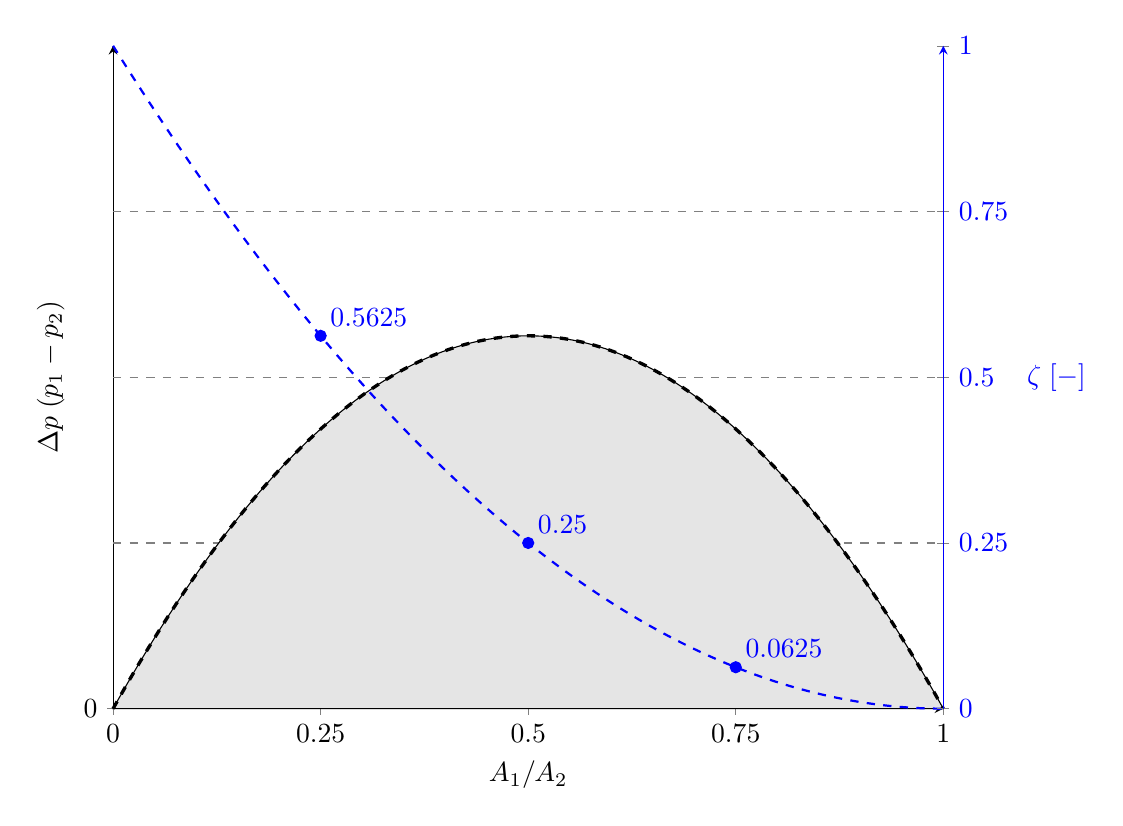
\begin{tikzpicture}
      %
      % Left axis (Δp)
      \begin{axis}[
        name=left,
        width=\textwidth, height=10cm,
        xmin=0, xmax=1,  ymin=0, ymax=1,
        axis x line=bottom,
        axis y line=left,
        every axis x line/.append style={-stealth},
        every axis y line/.append style={-stealth},
        xlabel={$A_1/A_2$},
        ylabel={$\displaystyle\Delta p\;(p_1-p_2)$},
        xtick={0,0.25,0.5,0.75,1},
        ytick={0},            % only label y=0 on left
        clip=false,
      ]
        % guide lines
        \draw[gray,dashed] (axis cs:0,0.25) -- (axis cs:1,0.25);
        \draw[gray,dashed] (axis cs:0,0.50) -- (axis cs:1,0.50);
        \draw[gray,dashed] (axis cs:0,0.75) -- (axis cs:1,0.75);
        \draw[gray,dashed] (axis cs:0.5,0) -- (axis cs:0.5,0.5625);
    
        % shaded area under black parabola
        \addplot [
          domain=0:1,
          samples=200,
          fill=black!10, 
        ] ({x},{-2.25*(x-0.5)^2+0.5625}) \closedcycle;
    
        % black dashed parabola
        \addplot [
          domain=0:1,
          samples=200,
          black,dashed,
          very thick,
        ] { -2.25*(x-0.5)^2 + 0.5625 };
    
        % blue dashed zeta‐curve
        \addplot [
          domain=0:1,
          samples=200,
          blue,dashed,
          thick,
        ] { (1 - x)^2 };
    
        % marked sample points on zeta‐curve
        \addplot [blue, only marks, mark=*, mark size=2pt] 
          coordinates {
            (0.25,0.5625) (0.5,0.25) (0.75,0.0625)
          };
    
        % point labels
        \node[blue, above right] at (axis cs:0.25,0.5625) {0.5625};
        \node[blue, above right] at (axis cs:0.5,0.25) {0.25};
        \node[blue, above right] at (axis cs:0.75,0.0625) {0.0625};
      \end{axis}
    
      %
      % Right axis (ζ)
      \begin{axis}[
        at={(left.north east)},
        anchor=north east,
        width=10cm, height=10cm,
        xmin=0, xmax=1,  ymin=0, ymax=1,
        axis x line=none,
        axis y line={right, blue},
        every axis y line/.append style={-stealth,blue},
        ytick={0,0.25,0.5,0.75,1},
        yticklabels={0,0.25,0.5,0.75,1},
        ylabel={$\zeta\;[-]$},
        ylabel style={blue, rotate=270},
      ]\end{axis}
    
    \end{tikzpicture}
\end{center}

\newpage
\subsubsection{Energy diagram}
\begin{center}
    \includegraphics[width=\textwidth]{media/energy_diagramm_angular.png}
\end{center}

\subsection{Second application of the angular momentum equation}
\subsubsection{Mixing losses}
\begin{center}
    \includegraphics[width=.75\textwidth]{media/mixing_losses.png}
\end{center}
















\end{document}
